\documentclass[10pt,a4paper]{article}
\usepackage[utf8]{inputenc}
\usepackage[english]{babel}
\usepackage[T1]{fontenc}
\usepackage{amsmath}
\usepackage{amsfonts}
\usepackage{amssymb}
\usepackage{graphicx}
\usepackage{listings}
\author{Milan Tepic, Ivan Antunovic, Peter von Zameck Glyscinski}
\title{Assignment 4 Team 5}
\bibliographystyle{plain}

\begin{document}
\maketitle
\section*{Task 1}
\subsection*{a)}
\begin{figure}[h]
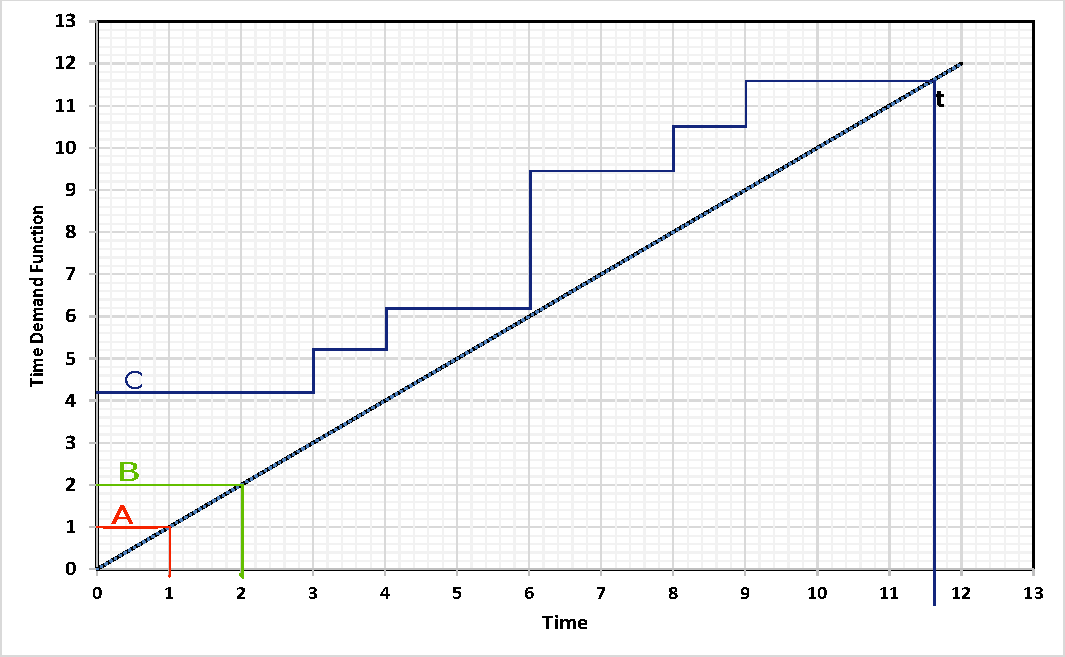
\includegraphics[width=\linewidth]{time-demand-1a.pdf}
\caption{Time demand diagram.} 
\label{fig:1a}
\end{figure}

\subsection*{b)}

\begin{figure}[h]
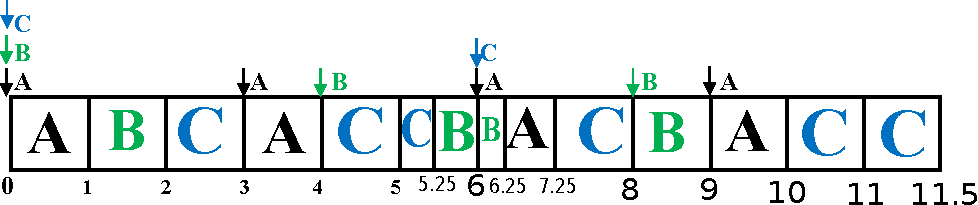
\includegraphics[width=\linewidth]{1b-edf.pdf}
\caption{Timming diagramm with edf.} 
\label{fig:1bedf}
\end{figure}

\begin{figure}[h]
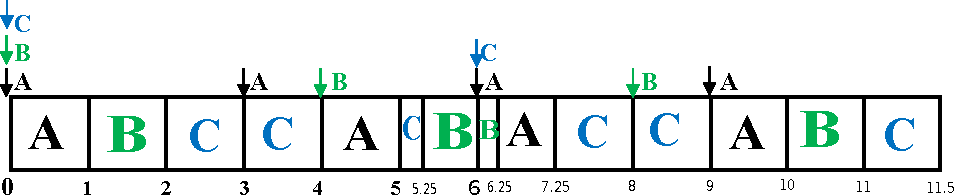
\includegraphics[width=\linewidth]{1b-lst.pdf}
\caption{Timming diagramm with lst.} 
\label{fig:1blst}
\end{figure}

\subsection*{c)}

\begin{figure}[h]
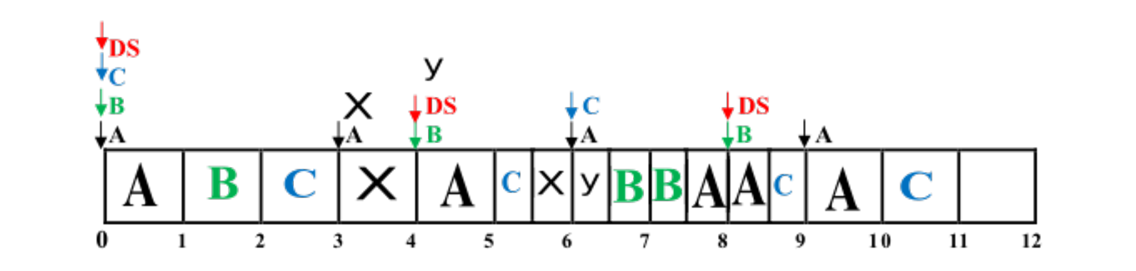
\includegraphics[width=\linewidth]{1c.pdf}
\caption{Timming diagramm with aperiodic tasks.} 
\label{fig:1c}
\end{figure}
\newpage

\section*{Task 2}
\subsection*{a)}
\begin{tabular}{|c|c|c|c|}
\hline
    Context & Timer 1 & Timer 2 & Timer 3 \\
    \hline
    Context 1 & $\overline{w_{39}}$ ~in ~$i_4$ & $\overline{w_{51}}$ ~in ~$i_4$ & $\overline{w_0}$ ~in ~$i_4$ \\
    \hline
    Context 2 & $\overline{w_{9}}$ ~in ~$i_1$ &  $\overline{w_{51}}$ ~in ~$i_4$ & $\overline{w_0}$ ~in ~$i_4$ \\
    \hline
    Context 3 & - &  $\overline{w_{51}}$ ~in ~$i_4$ & $\overline{w_0}$ ~in ~$i_4$ \\
    \hline
    Context 4 & - & - &  $\overline{w_{27}}$ ~in ~$i_3$\\
    \hline
\end{tabular}


\end{document}